\documentclass[12pt]{article}
\usepackage[utf8]{inputenc}
\usepackage{graphicx}
\usepackage[a4paper,width=150mm,top=25mm,bottom=25mm]{geometry}
\usepackage{float}

\title{
{
\includegraphics[width=4.5cm, height=4.5cm]{Figs/logo-uit-300x248.png}
}
\\
{Software requirement specification document for Football League Managementproject}
}



\author{Hoang Tan, Tien Dat, Duy Ngo \\ Supervised by Lecture: Nguyen Thi Thanh Truc }

\begin{document}

\maketitle
\tableofcontents
\section{Introduction}
\subsection{Purpose of this document}
The purpose of this Software Requirements Specification (SRS) document is to provide a detailed description of the requirements for the development of a Football League Management App using ASP.net. This document will serve as a guide for the developers and stakeholders involved in the project, outlining the functional and non-functional requirements of the app.

The SRS document will help to ensure that everyone involved in the project is on the same page, and that the app meets the expectations of all stakeholders. It will also help to minimize misunderstandings and errors that could arise during the development process by providing a clear, concise description of the app's features, functionality, and constraints.

The SRS document will be used throughout the development process as a reference for the developers and stakeholders, and will be used to validate that the completed app meets the requirements outlined in the document.

Overall, the purpose of this document is to provide a comprehensive description of the Football League Management App, including its features, functionality, and requirements, to ensure a successful development process and a high-quality, user-friendly final product.
\subsection{ Scope of this document}
The scope of this document includes the functional and non-functional requirements of the app, as well as any constraints, assumptions, and dependencies that must be taken into account during the development process. The document is intended for use by the development team, stakeholders, and other interested parties, and is meant to provide a clear and detailed description of the app's features and functionality.

The scope of this document does not include detailed design specifications or implementation details, but rather provides a high-level overview of the app's requirements. It is intended to be used as a reference throughout the development process, to ensure that the app meets the needs of all stakeholders and functions as expected.

Overall, the scope of this document is to provide a clear and detailed description of the requirements for the development of the Football League Management App, to guide the development team and stakeholders throughout the project, and to ensure a successful and high-quality final product.
\subsection{Overview}
The Football League Management App is a web-based application developed using ASP.net, designed to provide a comprehensive solution for managing a football league. The app will allow users to manage clubs, fixtures, results, rankings, notifications, and finances, and will provide clubs with the ability to manage their own information.

The app will be designed with a user-friendly interface, allowing for easy navigation and use. The app will be accessible through a web browser and will be compatible with desktop and mobile devices.

The main features of the app will include:
\begin{itemize}
    \item User registration and login
    \item Ability to manage clubs, including creating, updating, promoting, demoting, and deleting clubs
    \item Ability to manage fixtures, including scheduling, updating, and cancelling fixtures
    \item Ability to manage results and rankings, including updating and displaying league tables
    \item Ability to send notifications and documentation to all clubs
    \item Ability to manage finances of the league, including tracking income and expenses and generating financial reports
    \item Ability to penalize clubs for infringements
    \item Ability to manage a prize pool for high achieving clubs and outstanding players
    \item Ability for clubs to manage their own information, including updating their profiles and managing their players
\end{itemize}
The app will be developed with a focus on performance, scalability, security, and usability. It will be designed to handle a large volume of data and users, and will be secured with appropriate measures to protect sensitive information.

Overall, the Football League Management App will provide a comprehensive and user-friendly solution for managing a football league, streamlining administrative tasks and improving communication between clubs and league administrators.
\subsection{ Business Context}
The development of the Football League Management App is a university project aimed at providing a comprehensive and efficient solution for managing football leagues.

The project recognizes the importance of technology in achieving these goals and aims to leverage the latest technological advancements to develop a state-of-the-art solution for managing football leagues. The Football League Management App is a key component of the project's strategy for achieving its goals, and the development of the app is a top priority for the project.



\section{General Description}
\subsection{Product Functions}

The Football League Management App is a web-based application that aims to provide a comprehensive solution for managing football leagues. The app will allow league administrators to manage all aspects of the league, including clubs, fixtures, results, and rankings. It will also provide clubs with a platform to manage their own information and track their progress.

The key functions of the Football League Management App are as follows:
\begin{itemize}
    \item Sign up: The app will allow league administrators and clubs to create their own accounts and sign up for the league.

    \item Login: Once signed up, users will be able to log in to the app and access their respective accounts.

    \item Change password: Users will be able to change their passwords at any time, for security purposes.

    \item Manage all clubs: League administrators will be able to manage all clubs participating in the league, including adding, editing, and deleting clubs.

    \item Result and ranking management: The app will allow league administrators to manage results and rankings for each fixture, as well as for the overall league standings.

    \item Promote, demote, delete clubs: League administrators will be able to promote or demote clubs to different leagues based on their performance, or remove them from the league altogether.

    \item Notification and documentation to all clubs: The app will provide a platform for league administrators to communicate with all clubs, as well as share important documents and information.

    \item Schedule fixture: League administrators will be able to schedule fixtures for each round of the league, including specifying the date, time, and location of the fixture.

    \item Penalize for infringement: The app will provide a mechanism for league administrators to penalize clubs for infringements, such as misconduct or breach of rules.

    \item Manage finance of the league: The app will allow league administrators to manage the financial aspects of the league, including setting and collecting fees, managing expenses, and distributing prizes.

    \item Prize pool for high achievement clubs and outstanding players: The app will provide a platform for league administrators to manage a prize pool for high-achieving clubs and outstanding players, based on performance metrics and other criteria.

    \item Manage own club: Clubs will be able to manage their own information, including player rosters, game schedules, and performance metrics.
\end{itemize}

Overall, the Football League Management App will provide a comprehensive solution for managing football leagues, with features designed to streamline administrative tasks, improve communication, and promote fair play and transparency.
\subsection{Similar System Information}
There are several other football league management systems available in the market, including both commercial and open-source solutions. However, most of these systems are either too complex and difficult to use, or lack key features that are essential for effective league management.

The Football League Management App is intended to be a stand-alone product, designed to provide a comprehensive solution for managing football leagues. It is not intended to be used as a component of a larger product. However, the app will be compatible with other systems and software, allowing users to import and export data as needed.
\subsection{ User Characteristics}
The Football League Management App is designed to be used by two primary user groups:
\begin{itemize}
    \item League Administrators: These users are expected to have a high level of expertise in football league management and should be familiar with software systems commonly used for managing leagues. They will be responsible for setting up and configuring the app, managing league settings, and monitoring league activity.

    \item Clubs: These users may have varying levels of expertise with software systems, but should have a basic understanding of how to use computers and mobile devices. They will use the app to manage their club, including adding and editing player and staff profiles, submitting results and fixtures, and tracking their finances.
\end{itemize}
Both user groups are expected to have a basic understanding of the football league domain, including rules and regulations, and common terminology used in league management.

The app will be designed with a user-friendly interface and will include help documentation and tutorials to assist users with common tasks. In addition, support will be available to help users with any questions or issues they may encounter while using the app.

Overall, the Football League Management App is designed to be accessible and easy to use for users of varying levels of expertise, with features and functionality tailored to the specific needs of league administrators and clubs.
\subsection{ User Problem Statement}
The user community for the Football League Management App faces several key challenges when managing football leagues:
\begin{itemize}
    \item Lack of comprehensive solutions: Many existing football league management systems are either too complex or lack key features required for effective league management. This often leads to frustration and inefficiencies for league administrators and clubs.

    \item Inefficient manual processes: Without a comprehensive software solution, many league administrators and clubs resort to using manual processes to manage their leagues. This can be time-consuming and error-prone, leading to inaccuracies in results and rankings.

    \item Poor communication and collaboration: With manual processes, it can be difficult for league administrators and clubs to effectively communicate and collaborate with each other. This can lead to misunderstandings, missed deadlines, and a lack of transparency in league activities.

    \item Limited access: Without mobile-friendly solutions, league administrators and clubs may be limited in their ability to manage leagues on-the-go. This can be particularly challenging for clubs, who may need to submit results and fixtures while on the road for away games.
\end{itemize}
The Football League Management App aims to address these challenges by providing a comprehensive, user-friendly solution for managing football leagues. With a range of features and functionality designed specifically for league management, the app is expected to improve efficiency, communication, and collaboration between league administrators and clubs, while providing greater accessibility and flexibility for users.
\subsection{ User Objectives}
The user community for the Football League Management App has several key objectives for the system:
\begin{itemize}
    \item Comprehensive league management: The app should provide a comprehensive solution for managing all aspects of a football league, including setting up league rules and settings, managing club and player profiles, submitting results and fixtures, and managing league finances.

    \item User-friendly interface: The app should have a user-friendly interface that is easy to navigate and use, with clear and concise instructions for common tasks.

    \item Mobile accessibility: The app should be accessible on mobile devices, allowing users to manage their leagues on-the-go.

    \item Efficient and accurate processes: The app should streamline league management processes, reducing the need for manual processes and minimizing the risk of errors and inaccuracies.

    \item Effective communication and collaboration: The app should facilitate effective communication and collaboration between league administrators and clubs, with features such as notifications, messaging, and shared documents.

    \item Customizable settings: The app should allow league administrators to customize league settings and rules to fit their specific needs.

    \item Security and privacy: The app should ensure the security and privacy of user data, with features such as password protection and data encryption.

    \item Affordable pricing: The app should be priced at an affordable level for both small and large leagues, with transparent pricing and no hidden fees.
\end{itemize}
Overall, the Football League Management App aims to meet these user objectives by providing a comprehensive, user-friendly solution for managing football leagues, with a range of features and functionality designed to improve efficiency, communication, and collaboration between league administrators and clubs.

\subsection{ General Constraints}
The design and development of the Football League Management App is subject to the following general constraints:
\begin{itemize}
    \item Hardware and software platforms: The app must be designed to run on common hardware and software platforms, including desktop and mobile devices running Windows, MacOS, iOS, and Android operating systems.

    \item Speed and performance: The app must be designed to provide fast and efficient performance, with minimal lag time or delays when loading or processing data.

    \item Security and privacy: The app must be designed to ensure the security and privacy of user data, with features such as password protection, data encryption, and secure data storage.

    \item Industry protocols and standards: The app must comply with relevant industry protocols and standards, including those related to data privacy, security, and accessibility.

    \item User interface and experience: The app must be designed to provide a user-friendly interface and experience, with clear and concise instructions for common tasks, and intuitive navigation.

    \item Budget constraints: The design and development of the app must be completed within a specific budget, with careful consideration given to the cost of development tools, hardware and software platforms, and ongoing maintenance and support.
\end{itemize}
Overall, the Football League Management App must be designed and developed within these general constraints to ensure its success as a comprehensive and user-friendly solution for managing football leagues.


\section{Functional Requirements}



% Please add the following required packages to your document preamble:
% \usepackage{graphicx}



\begin{table}[H]
    \caption{Functional Requirement Sign Up}
    \label{tab:signup-table}
    \resizebox{\textwidth}{!}{%
    \begin{tabular}{|l|l|}
    \hline
    Function Name                        & Sign up                                                                                            \\ \hline
    Description                          & Users must be able to create an account by entering their basic personal information such as name, email address, and password.                                                                                                                               \\ \hline
    Critically                           & Must have

    \\ \hline
    Technical issues                     &  Implementing a secure password encryption algorithm to ensure the security of user data.                                                                               \\ \hline
    Cost and schedule                    & Low cost and minimal time are required to implement this function.                                                                                                 \\ \hline
    Risks                                & The risk of creating a weak password, which could result in the user's account being compromised. This risk can be minimized by enforcing a password complexity policy. \\ \hline
    Pre-Condition                        & The user must be on the registration page of the platform.                                                                                                           \\ \hline
    Post-Condition                       &  The user's account is created, and they are automatically logged in to the platform.                                                                                                                \\ \hline
    \end{tabular}%
    }
\end{table}

\begin{table}[H]
    \caption{Functional Requirement Login}
    \label{tab:login-table}
    \resizebox{\textwidth}{!}{%
    \begin{tabular}{|l|l|}
    \hline
    Function Name                        & Login                                                                                            \\ \hline
    Description                          & Users must be able to log in to the platform by entering their email and password.                                                                                                                               \\ \hline
    Critically                           & Must have                                                                                                   \\ \hline
    Technical issues                     & Ensuring the authentication process is secure and that the user's login information is not vulnerable to unauthorized access.                                                                               \\ \hline
    Cost and schedule                    & Low cost and minimal time are required to implement this function.                                                                                                 \\ \hline
    Risks                                & The risk of unauthorized access to the user's account. This risk can be minimized by enforcing strict security policies and implementing multi-factor authentication. \\ \hline

    Pre-Condition                        & The user must have an existing account on the platform.                                                                                                           \\ \hline
    Post-Condition                       & The user is logged in to their account and can access the platform's functionalities.                                                                                                                \\ \hline
    \end{tabular}%
    }
    \end{table}

    \begin{table}[H]
        \caption{Functional Requirement Change password}
        \label{tab:changepwd-table}
        \resizebox{\textwidth}{!}{%
        \begin{tabular}{|l|l|}
        \hline
        Function Name                        & Change password                                                                                            \\ \hline
        Description                          & Users must be able to change their password for security purposes.                                                                                                                               \\ \hline
        Critically                           & Important.                                                                                                   \\ \hline
        Technical issues                     & Ensuring the password change process is secure and that the user's new password is not vulnerable to unauthorized access.                                                                               \\ \hline
        Cost and schedule                    & Low cost and minimal time are required to implement this function.                                                                                                 \\ \hline
        Risks                                & The risk of forgetting the new password or creating a weak password. This risk can be minimized by providing password complexity requirements and implementing password reset functionality. \\ \hline

        Pre-Condition                        & The user must be logged in to their account.                                                                                                           \\ \hline
        Post-Condition                       & The user's password is changed, and they are required to log in again using their new password.                                                                                                                \\ \hline
        \end{tabular}%
        }
        \end{table}


        \begin{table}[H]
            \caption{Functional Requirement Manage all clubs}
            \label{tab:manageall-table}
            \resizebox{\textwidth}{!}{%
            \begin{tabular}{|l|l|}
            \hline
            Function Name                        & Manage all clubs                                                                                            \\ \hline
            Description                          & Allow authorized users to manage all the clubs in the football league by adding new clubs, updating existing ones, and deleting inactive clubs.                                                                                                                               \\ \hline
            Critically                           & Essential                                                                                                   \\ \hline
            Technical issues                     & Proper access control mechanisms should be implemented to ensure that only authorized users can manage clubs.                                                                               \\ \hline
            Cost and schedule                    & Medium                                                                                                 \\ \hline
            Risks                                & The risk of unauthorized access to club management functions can be mitigated by implementing proper access control measures. \\ \hline

            Pre-Condition                        & The user is authorized to manage clubs in the system.                                                                                                          \\ \hline
            Post-Condition                       & The club information is updated or a new club is added or inactive clubs are deleted.                                                                                                                \\ \hline
            \end{tabular}%
            }
            \end{table}

            \begin{table}[H]
                \caption{Functional Requirement Promote, demote, delete clubs}
                \label{tab:pdd-table}
                \resizebox{\textwidth}{!}{%
                \begin{tabular}{|l|l|}
                \hline
                Function Name                        & Promote, demote, delete clubs                                                                                            \\ \hline
                Description                          & Allow authorized users to promote, demote, or delete clubs based on their performance in the league.                                                                                                                               \\ \hline
                Critically                           & Essential                                                                                                 \\ \hline
                Technical issues                     & Proper access control mechanisms should be implemented to ensure that only authorized users can promote, demote, or delete clubs.                                                                         \\ \hline
                Cost and schedule                    & Medium                                                                                                \\ \hline
                Risks                                & The risk of incorrect promotions or demotions can be mitigated by implementing proper validation mechanisms. \\ \hline

                Pre-Condition                        & The user is authorized to promote, demote, or delete clubs in the system.                                                                                                           \\ \hline
                Post-Condition                       & Clubs are promoted, demoted, or deleted according to the user's actions.

                                                                                                                            \\ \hline
                \end{tabular}%
                }
                
                \end{table}
\begin{table}[H]
                    \caption{Functional Requirement Manage Results and Rankings}
                    \label{tab:result-ranking-table}
                    \resizebox{\textwidth}{!}{%
                    \begin{tabular}{|l|l|}
                    \hline
                    Function Name                        & Manage Results and Rankings                                                                                            \\ \hline
                    Description                          & This function allows the league manager to input the results of matches played by the various clubs and automatically generates an up-to-date ranking table based on the results.                                                                                                                               \\ \hline
                    Critically                           & Must have
                
                    \\ \hline
                    Technical issues                     &  The technical issues involved in implementing this requirement include designing a user-friendly interface for inputting match results, implementing an algorithm that accurately calculates the ranking of each club based on the results of their matches, and ensuring that the ranking table is displayed correctly.                                                                               \\ \hline
                    Cost and schedule                    & The cost and schedule of implementing this requirement depend on the complexity of the algorithm used for ranking clubs and the amount of time required to design and test the user interface.

                    \\ \hline
                    Risks                                & The main risk associated with this requirement is the potential for inaccuracies in the ranking system due to incorrect data input by the league manager. 

                    \\ \hline
                    Pre-Condition                        & The league manager has logged into the system and has access to the match results.                                                                                                           \\ \hline
                    Post-Condition                       &  The system generates an updated ranking table based on the inputted match results.                                                                                                                \\ \hline
                    \end{tabular}%
                    }
\end{table}    

\begin{table}[H]
    \caption{Functional Requirement Send notification and documentation to all clubs}
    \label{tab:noti-doc-table}
    \resizebox{\textwidth}{!}{%
    \begin{tabular}{|l|l|}
    \hline
    Function Name                        & Send notification and documentation to all clubs.                                                                                            \\ \hline
    Description                          & The system should allow the league administrator to send notifications and documentation (such as rule changes, meeting minutes, etc.) to all registered clubs.                                                                                                                               \\ \hline
    Critically                           & Important.                                                                                                   \\ \hline
    Technical issues                     & The system will need to implement a messaging system that allows for the creation and sending of messages to all registered clubs.                                                                                \\ \hline
    Cost and schedule                    & The cost and schedule of implementing this function will depend on the complexity of the messaging system and the desired features                                                                                                 \\ \hline
    Risks                                &  There is a risk that messages may not be delivered or may be overlooked by clubs.                                                                                                                      \\ \hline
    Pre-Condition                        & The league administrator must be logged into the system and have authorization to send messages to all clubs.                                                                                                           \\ \hline
    Post-Condition                       & All registered clubs should receive the message and be able to access it in their message inbox or notification center.                                                                                                                \\ \hline
    \end{tabular}%
    }
    \end{table}

    \begin{table}[H]
        \caption{Functional Requirement Schedule fixture}
        \label{tab:schedule-table}
        \resizebox{\textwidth}{!}{%
        \begin{tabular}{|l|l|}
        \hline
        Function Name                        & Schedule fixture                                                                                           \\ \hline
        Description                          & Allows the league administrator to schedule fixtures between clubs and update the schedule as needed.                                                                                                                               \\ \hline
        Critically                           & crucial                                                                                                   \\ \hline
        Technical issues                     & The system must be able to handle conflicting schedules and ensure that no club is scheduled to play two matches at the same time or on the same day.                                                                               \\ \hline
        Cost and schedule                    & The cost and schedule of this function will depend on the complexity of the scheduling algorithm used and the frequency of updates required.                                                                                                  \\ \hline
        Risks                                & The risk of this function not being able to be satisfied is low, as there are existing scheduling algorithms that can be used. \\ \hline

        Pre-Condition                        & The league administrator must have access to all necessary information regarding club availability, stadium availability, and any other relevant scheduling constraints.                                                                                                           \\ \hline
        Post-Condition                       & A schedule is generated that assigns each club to a specific time and place for each match, and all clubs are notified of their scheduled matches.                                                                                                                \\ \hline
        \end{tabular}%
        }
    \end{table}
        \begin{table}[H]
            \caption{Functional Requirement Penalize for infringement}
            \label{tab:penalize-table}
            \resizebox{\textwidth}{!}{%
            \begin{tabular}{|l|l|}
            \hline
            Function Name                        & Penalize for infringement.                                                                                            \\ \hline
            Description                          & The system should allow the league administrators to impose penalties on clubs or players who violate the league rules.                                                                                                                               \\ \hline
            Critically                           & Medium                                                                                                   \\ \hline
            Technical issues                     & The system needs to have a mechanism to track violations and penalties and display them publicly to ensure transparency.                                                                                \\ \hline
            Cost and schedule                    & The cost of implementing this requirement may depend on the complexity of the penalty system and the level of automation required.                                                                                                  \\ \hline
            Risks                                & There is a risk of incorrectly imposing penalties or not imposing penalties when necessary. \\ \hline

            Pre-Condition                        & The league rules and regulations should be clearly defined and communicated to all clubs and players.                                                                                                           \\ \hline
            Post-Condition                       & The penalties imposed should be recorded and reflected in the standings and rankings.                                                                                                                \\ \hline
            \end{tabular}%
            }
            \end{table}     
            \begin{table}[H]
                \caption{Functional Requirement Manage finance of the league}
                \label{tab:club-finance-table}
                \resizebox{\textwidth}{!}{%
                \begin{tabular}{|l|l|}
                \hline
                Function Name                        & Manage finance of the league                                                                                            \\ \hline
                Description                          & The system should allow the league administrators to manage the financial aspects of the league, including revenue generation, expenses, and budgeting.                                                                                                                               \\ \hline
                Critically                           & Medium.                                                                                                   \\ \hline
                Technical issues                     & The system needs to have a mechanism to track revenue and expenses and generate financial reports.                                                                                \\ \hline
                Cost and schedule                    & The cost of implementing this requirement will depend on the complexity of the financial management system.                                                                                                  \\ \hline
                Risks                                & There is a risk of financial mismanagement or fraud. To reduce this risk, the system should have appropriate controls and audit trails in place. \\ \hline
 
                Pre-Condition                        & The league administrators should have a clear understanding of the league's financial goals and objectives.                                                                                                          \\ \hline
                Post-Condition                       & The financial records should be accurate and up-to-date, and the league should be able to operate within its budget.                                                                                                                \\ \hline
                \end{tabular}%
                }
                \end{table}  
                \begin{table}[H]
                    \caption{Functional Requirement Prize pool for high achievement clubs and outstanding players}
                    \label{tab:prize-pool-table}
                    \resizebox{\textwidth}{!}{%
                    \begin{tabular}{|l|l|}
                    \hline
                    Function Name                        & Prize pool for high achievement clubs and outstanding players                                                                                            \\ \hline
                    Description                          & The system should allow the league administrators to create a prize pool for high-achieving clubs and outstanding players.                                                                                                                            \\ \hline
                    Critically                           & Important                                                                                                   \\ \hline
                    Technical issues                     & The system needs to have a mechanism to track performance and calculate rewards based on predefined criteria.                                                                               \\ \hline
                    Cost and schedule                    & The cost of implementing this requirement will depend on the size and complexity of the prize pool.                                                                                                 \\ \hline
                    Risks                                & There is a risk of unfairness or bias in the selection of winners. To reduce this risk, the criteria for selecting winners should be transparent and objective. \\ \hline

                    Pre-Condition                        & The criteria for selecting winners should be clearly defined and communicated to all clubs and players.                                                                                                           \\ \hline
                    Post-Condition                       & The rewards should be distributed fairly among eligible clubs and players.                                                                                                                \\ \hline
                    \end{tabular}%
                    }
                    \end{table}
                    \begin{table}[H]
                        \caption{Functional Requirement Manage own club}
                        \label{tab:manage-own-table}
                        \resizebox{\textwidth}{!}{%
                        \begin{tabular}{|l|l|}
                        \hline
                        Function Name                        & Manage own club                                                                                            \\ \hline
                        Description                          & Allows club owners to manage their club information, including club name, logo, players, coach, and staff. Club owners can add, edit, or remove players, coaches, and staff from their club.                                                                                                                            \\ \hline
                        Critically                           & essential                                                                                                   \\ \hline
                        Technical issues                     & The system needs to ensure that club owners only have access to their club's information and cannot view or edit information about other clubs.                                                                               \\ \hline
                        Cost and schedule                    & The cost and schedule for implementing this function will depend on the complexity of the system and the number of features included.                                                                                                 \\ \hline
                        Risks                                & The risk involved with this function is that club owners may accidentally delete important information or make changes that negatively impact their club's performance.  \\ \hline
    
                        Pre-Condition                        & The club owner is logged in to the system and has access to their club's information.                                                                                                           \\ \hline
                        Post-Condition                       & The club owner has successfully managed their club's information and can view the changes made in the system.                                                                                                                \\ \hline
                        \end{tabular}%
                        }
                        \end{table}
\section{Interface Requirements} 
\subsection{User Interfaces}
The system will have a user interface that allows the league management and club management staff to perform various operations such as scheduling fixtures, managing finances, managing results and rankings, and managing players' data. The user interface will be developed using modern web technologies such as HTML, CSS, and JavaScript.
\subsubsection {GUI}
The Graphical User Interface (GUI) of the system is designed to provide an intuitive and user-friendly way for the user to interact with the system. The GUI provides a set of screens that allow the user to perform various functions such as managing clubs, players, fixtures, and results, as well as viewing league tables and player statistics. The GUI is designed with the following features:
\begin{itemize}
    \item Navigation Menu: The navigation menu provides access to all the different functionalities of the system. It includes options such as "Manage Club", "Manage Players", "Schedule Fixture", "View Results", "View League Table", "View Player Statistics", and so on.
    \item Input Forms: The system provides input forms to collect user inputs for various functionalities. The input forms are designed with input validation and error messages to ensure data integrity.
    \item Tables: The system displays data in tabular format for easy viewing and analysis. The tables are designed with sorting and filtering capabilities to allow the user to easily find and manipulate data.
    \item Charts: The system provides charts and graphs to display league tables and player statistics in a visually appealing and easy-to-understand format.
\end{itemize}
\subsubsection {Diagnostics or ROM}
The system shall have a built-in diagnostic feature that will help in the detection and correction of any errors in the software. When an error is encountered, the system will generate an error message that will be displayed on the user interface. The message will include the error code, a brief description of the error, and recommendations for resolving the issue.

The system will also maintain a log file that records all system events, including errors, warnings, and informational messages. This log file will be stored on the server and can be accessed by the system administrator for debugging and diagnostic purposes.

In addition, the system will provide a remote access feature that will allow the system administrator to remotely access the server for debugging and diagnostic purposes. The remote access feature will require authentication and authorization to ensure the security of the system.

The system will also include a ROM that contains the system software, data, and configuration files. This ROM will be used as a backup in case of system failure, and can be used to restore the system to its previous state. The ROM will be stored in a secure location and will be regularly updated to ensure the system is always backed up.

\subsection{Hardware Interfaces}
The Football League Management system does not have any direct interfaces to hardware devices. However, the system requires a computer or mobile device with internet connectivity to access and utilize the software. The system is compatible with a wide range of hardware devices, including desktop computers, laptops, tablets, and smartphones. Additionally, the system may utilize hardware devices such as printers to generate physical copies of reports or other data outputs. The system does not require any specific hardware configuration, but it is recommended that users utilize devices with modern hardware specifications to ensure optimal performance.
\subsection{Communications Interfaces}
The Football League Management system will require communication interfaces to various external systems and networks. These interfaces will include:
\begin{itemize}
    \item Internet Connectivity: The system will need to be connected to the Internet in order to access external data and information, such as real-time match scores, news updates, and other relevant data. This interface will need to support standard networking protocols such as TCP/IP, HTTP, and FTP.

    \item Email Notifications: The system will be capable of sending automated email notifications to club officials, referees, and other relevant parties, such as match schedules, results, and other updates. This interface will use standard email protocols such as SMTP and POP3.

    \item SMS Notifications: In addition to email, the system will also be capable of sending automated SMS notifications to club officials and other relevant parties. This interface will use standard SMS protocols such as SMPP.
\end{itemize}
Overall, the communication interfaces of the Football League Management system will need to be reliable, secure, and scalable to ensure that all relevant parties can access and interact with the system effectively.

\section{Performance Requirements}
The performance of the system is critical for efficient management of the football league. The system must meet the following requirements:
\begin{itemize}
    \item Response Time: The system must have a response time of less than 2 seconds for all user interactions.

    \item Scalability: The system must be able to handle a large number of users and data without any performance degradation.

    \item Memory usage: The system must be optimized to use the minimum amount of memory possible.

    \item Reliability: The system must be reliable and have an uptime of at least 99.9%.

    \item Security: The system must be secured from any external threats and must have a proper authentication mechanism to ensure the safety of data.
\end{itemize}
\section{Design Constraints}
\begin{itemize}
    \item Technology: The system will be developed using ASP.NET, and the design team must ensure that all modules and components are compatible with this technology.

    \item Platform: The system must be compatible with the Windows operating system and run on the .NET framework. The design team must ensure that all modules and components are compatible with the specified platform.

    \item Security: The system must provide secure access to the database and other critical resources. The design team must implement security measures such as authentication, authorization, and encryption to ensure data confidentiality and integrity.

    \item Performance: The system must perform efficiently and handle a large number of concurrent users. The design team must optimize the system performance by minimizing response time, network latency, and resource usage.

    \item Scalability: The system must be scalable and able to handle an increase in the number of users and data volume. The design team must ensure that the system architecture and database design can support future expansion.

    \item Usability: The system must be user-friendly and easy to navigate. The design team must ensure that the user interface is intuitive and conforms to established usability standards.

    \item Accessibility: The system must comply with accessibility guidelines to ensure that users with disabilities can access and use the system. The design team must ensure that the user interface is compatible with assistive technologies and that all content is accessible to users with disabilities.

    \item Documentation: The design team must provide comprehensive documentation that includes technical specifications, design documents, user manuals, and installation guides. The documentation must be complete, accurate, and up-to-date.
\end{itemize}


\section{Other non-functional attributes}
The following non-functional attributes are also important for the system:
\begin{itemize}
    \item Security: The system must be designed with appropriate security measures to prevent unauthorized access, data breaches, and malicious attacks. User authentication and access control must be implemented to ensure that only authorized users can access sensitive data.
    \item Scalability: The system must be designed to handle a large number of users and a growing amount of data. It should be scalable and able to handle increasing demands without any significant performance degradation.
    \item Availability: The system must be highly available and accessible at all times. It should have a robust disaster recovery plan in place to ensure business continuity in the event of any system failures or disruptions.
    \item Reliability: The system must be reliable and consistent in its performance. It should minimize the occurrence of errors and ensure that data is accurately and consistently stored and retrieved.
    \item Usability: The system must be easy to use and navigate for all types of users, regardless of their technical expertise. It should have a user-friendly interface and clear documentation to support users in using the system.
    \item Maintainability: The system must be easy to maintain and update over time. It should be designed with modularity in mind, using standard coding practices and programming languages to facilitate maintenance and updates.
\end{itemize}

\section{Operational Scenarios}
Scenario 1: User Registration
John, a football enthusiast, wants to join the football league management system to register his team. John navigates to the registration page and enters his personal details and team information. The system verifies his information and creates a new user account. John logs in to the system and accesses his team dashboard.

Scenario 2: Fixture Schedule
As the league administrator, Maria wants to schedule fixtures for the upcoming season. Maria logs into the system and navigates to the fixture scheduling page. She selects the teams that will participate in each fixture and assigns the dates and times. The system validates the scheduling conflicts and confirms the fixtures.

Scenario 3: Penalty Issuance
As the referee of a football match, Tom notices a player from one of the teams violating a league rule. Tom records the incident in the system, and the system issues a penalty against the player and notifies the team management.

Scenario 4: Payment Processing
As the owner of a football team, Mark wants to pay the league fees for his team. Mark logs into the system and navigates to the payment processing page. He selects the payment method, enters the payment details, and confirms the payment. The system verifies the payment and updates Mark's team's account balance.

Scenario 5: Player Statistics
As the coach of a football team, Sarah wants to view the performance statistics of her team's players. Sarah logs into the system and navigates to the player statistics page. She selects the players whose statistics she wants to view and accesses their performance history. The system presents the statistics in an easy-to-understand format.

These scenarios provide a practical view of how the system will work in real-world scenarios. By using these scenarios, we can test the system's functionality and ensure that it meets the requirements of the stakeholders.

\section{Preliminary Object-Oriented Domain Analysis}

% \subsection{Inheritance Relationships}
% This section should contain a set of graphs that illustrate the primary inheritance hierarchy (is-kind-of) for the system. For example: 

\begin{figure}[H]
\centering
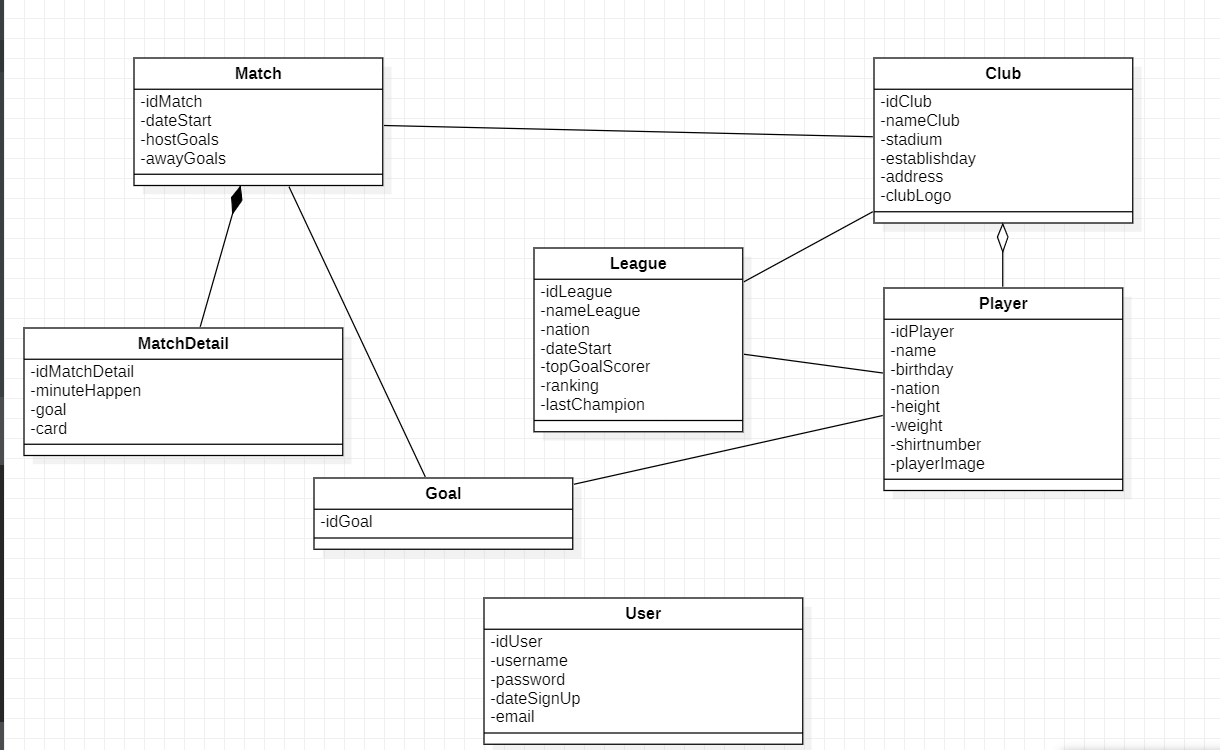
\includegraphics[scale=0.4]{Figs/Class.png}
\caption{Class diagram}
\label{fig:image}
\end{figure}
% \subsection{Class descriptions}
% This section presents a more detailed description of each class identified during the OO Domain Analysis. For more details on the process giving rise to these descriptions, see Lecture 5.3: OO Domain Analysis and/or texts on object-oriented software development. 
% Each class description should conform to the following structure: 
% \subsubsection{ Class name}
%  Abstract or Concrete: 
% Indicates whether this class is abstract or concrete. 
% \subsubsection {List of Superclasses:} 
% Names all immediate superclasses. 
% \subsubsection {List of Subclasses:} 
% Names all immediate subclasses. 
% \subsubsection {Purpose: }
% States the basic purpose of the class. 
% \subsubsection {Collaborations: }
% Names each class with which this class must interact in order to accomplish its purpose, and how. 
% \subsubsection {Attributes: }
% Lists each attribute (state variable) associated with each instance of this class, and indicates examples of possible values (or a range). 
% \subsubsection {Operations}: 
% Lists each operation that can be invoked upon instances of this class. For each operation, the arguments (and their type), the return value (and its type), and any side effects of the operation should be specified. 
% \subsubsection {Constraints:} 
% Lists any restrictions upon the general state or behavior of instances of this class. 



% \section{Preliminary Schedule Adjusted}
% This section provides an initial version of the project plan, including the major tasks to be accomplished, their interdependence's, and their tentative start/stop dates. The plan also includes information on hardware, software, and  resource requirements. 
% The project plan should be accompanied by one or more PERT or GANTT charts. 
% \section{Preliminary Budget Adjusted}
% This section provides an initial budget for the project, itemized by cost factor. 


\bibliographystyle{IEEEtranS}

\bibliography{dissertationbib}

\end{document}
